% Options for packages loaded elsewhere
\PassOptionsToPackage{unicode}{hyperref}
\PassOptionsToPackage{hyphens}{url}
\PassOptionsToPackage{dvipsnames,svgnames,x11names}{xcolor}
%
\documentclass[
  letterpaper,
  DIV=11,
  numbers=noendperiod]{scrreprt}

\usepackage{amsmath,amssymb}
\usepackage{lmodern}
\usepackage{iftex}
\ifPDFTeX
  \usepackage[T1]{fontenc}
  \usepackage[utf8]{inputenc}
  \usepackage{textcomp} % provide euro and other symbols
\else % if luatex or xetex
  \usepackage{unicode-math}
  \defaultfontfeatures{Scale=MatchLowercase}
  \defaultfontfeatures[\rmfamily]{Ligatures=TeX,Scale=1}
\fi
% Use upquote if available, for straight quotes in verbatim environments
\IfFileExists{upquote.sty}{\usepackage{upquote}}{}
\IfFileExists{microtype.sty}{% use microtype if available
  \usepackage[]{microtype}
  \UseMicrotypeSet[protrusion]{basicmath} % disable protrusion for tt fonts
}{}
\makeatletter
\@ifundefined{KOMAClassName}{% if non-KOMA class
  \IfFileExists{parskip.sty}{%
    \usepackage{parskip}
  }{% else
    \setlength{\parindent}{0pt}
    \setlength{\parskip}{6pt plus 2pt minus 1pt}}
}{% if KOMA class
  \KOMAoptions{parskip=half}}
\makeatother
\usepackage{xcolor}
\setlength{\emergencystretch}{3em} % prevent overfull lines
\setcounter{secnumdepth}{5}
% Make \paragraph and \subparagraph free-standing
\ifx\paragraph\undefined\else
  \let\oldparagraph\paragraph
  \renewcommand{\paragraph}[1]{\oldparagraph{#1}\mbox{}}
\fi
\ifx\subparagraph\undefined\else
  \let\oldsubparagraph\subparagraph
  \renewcommand{\subparagraph}[1]{\oldsubparagraph{#1}\mbox{}}
\fi


\providecommand{\tightlist}{%
  \setlength{\itemsep}{0pt}\setlength{\parskip}{0pt}}\usepackage{longtable,booktabs,array}
\usepackage{calc} % for calculating minipage widths
% Correct order of tables after \paragraph or \subparagraph
\usepackage{etoolbox}
\makeatletter
\patchcmd\longtable{\par}{\if@noskipsec\mbox{}\fi\par}{}{}
\makeatother
% Allow footnotes in longtable head/foot
\IfFileExists{footnotehyper.sty}{\usepackage{footnotehyper}}{\usepackage{footnote}}
\makesavenoteenv{longtable}
\usepackage{graphicx}
\makeatletter
\def\maxwidth{\ifdim\Gin@nat@width>\linewidth\linewidth\else\Gin@nat@width\fi}
\def\maxheight{\ifdim\Gin@nat@height>\textheight\textheight\else\Gin@nat@height\fi}
\makeatother
% Scale images if necessary, so that they will not overflow the page
% margins by default, and it is still possible to overwrite the defaults
% using explicit options in \includegraphics[width, height, ...]{}
\setkeys{Gin}{width=\maxwidth,height=\maxheight,keepaspectratio}
% Set default figure placement to htbp
\makeatletter
\def\fps@figure{htbp}
\makeatother
\newlength{\cslhangindent}
\setlength{\cslhangindent}{1.5em}
\newlength{\csllabelwidth}
\setlength{\csllabelwidth}{3em}
\newlength{\cslentryspacingunit} % times entry-spacing
\setlength{\cslentryspacingunit}{\parskip}
\newenvironment{CSLReferences}[2] % #1 hanging-ident, #2 entry spacing
 {% don't indent paragraphs
  \setlength{\parindent}{0pt}
  % turn on hanging indent if param 1 is 1
  \ifodd #1
  \let\oldpar\par
  \def\par{\hangindent=\cslhangindent\oldpar}
  \fi
  % set entry spacing
  \setlength{\parskip}{#2\cslentryspacingunit}
 }%
 {}
\usepackage{calc}
\newcommand{\CSLBlock}[1]{#1\hfill\break}
\newcommand{\CSLLeftMargin}[1]{\parbox[t]{\csllabelwidth}{#1}}
\newcommand{\CSLRightInline}[1]{\parbox[t]{\linewidth - \csllabelwidth}{#1}\break}
\newcommand{\CSLIndent}[1]{\hspace{\cslhangindent}#1}

\usepackage{booktabs}
\usepackage{longtable}
\usepackage{array}
\usepackage{multirow}
\usepackage{wrapfig}
\usepackage{float}
\usepackage{colortbl}
\usepackage{pdflscape}
\usepackage{tabu}
\usepackage{threeparttable}
\usepackage{threeparttablex}
\usepackage[normalem]{ulem}
\usepackage{makecell}
\usepackage{xcolor}
\KOMAoption{captions}{tableheading}
\makeatletter
\makeatother
\makeatletter
\@ifpackageloaded{bookmark}{}{\usepackage{bookmark}}
\makeatother
\makeatletter
\@ifpackageloaded{caption}{}{\usepackage{caption}}
\AtBeginDocument{%
\ifdefined\contentsname
  \renewcommand*\contentsname{Table of contents}
\else
  \newcommand\contentsname{Table of contents}
\fi
\ifdefined\listfigurename
  \renewcommand*\listfigurename{List of Figures}
\else
  \newcommand\listfigurename{List of Figures}
\fi
\ifdefined\listtablename
  \renewcommand*\listtablename{List of Tables}
\else
  \newcommand\listtablename{List of Tables}
\fi
\ifdefined\figurename
  \renewcommand*\figurename{Figure}
\else
  \newcommand\figurename{Figure}
\fi
\ifdefined\tablename
  \renewcommand*\tablename{Table}
\else
  \newcommand\tablename{Table}
\fi
}
\@ifpackageloaded{float}{}{\usepackage{float}}
\floatstyle{ruled}
\@ifundefined{c@chapter}{\newfloat{codelisting}{h}{lop}}{\newfloat{codelisting}{h}{lop}[chapter]}
\floatname{codelisting}{Listing}
\newcommand*\listoflistings{\listof{codelisting}{List of Listings}}
\makeatother
\makeatletter
\@ifpackageloaded{caption}{}{\usepackage{caption}}
\@ifpackageloaded{subcaption}{}{\usepackage{subcaption}}
\makeatother
\makeatletter
\@ifpackageloaded{tcolorbox}{}{\usepackage[many]{tcolorbox}}
\makeatother
\makeatletter
\@ifundefined{shadecolor}{\definecolor{shadecolor}{rgb}{.97, .97, .97}}
\makeatother
\makeatletter
\makeatother
\ifLuaTeX
  \usepackage{selnolig}  % disable illegal ligatures
\fi
\IfFileExists{bookmark.sty}{\usepackage{bookmark}}{\usepackage{hyperref}}
\IfFileExists{xurl.sty}{\usepackage{xurl}}{} % add URL line breaks if available
\urlstyle{same} % disable monospaced font for URLs
\hypersetup{
  pdftitle={Kenai Thermal Imagery},
  pdfauthor={Benjamin Meyer},
  colorlinks=true,
  linkcolor={blue},
  filecolor={Maroon},
  citecolor={Blue},
  urlcolor={Blue},
  pdfcreator={LaTeX via pandoc}}

\title{Kenai Thermal Imagery}
\author{Benjamin Meyer}
\date{11/18/22}

\begin{document}
\maketitle
\ifdefined\Shaded\renewenvironment{Shaded}{\begin{tcolorbox}[boxrule=0pt, borderline west={3pt}{0pt}{shadecolor}, enhanced, frame hidden, sharp corners, breakable, interior hidden]}{\end{tcolorbox}}\fi

\renewcommand*\contentsname{Table of contents}
{
\hypersetup{linkcolor=}
\setcounter{tocdepth}{2}
\tableofcontents
}
\bookmarksetup{startatroot}

\hypertarget{executive-summary}{%
\chapter*{Executive Summary}\label{executive-summary}}
\addcontentsline{toc}{chapter}{Executive Summary}

\markboth{Executive Summary}{Executive Summary}

\begin{figure}

{\centering 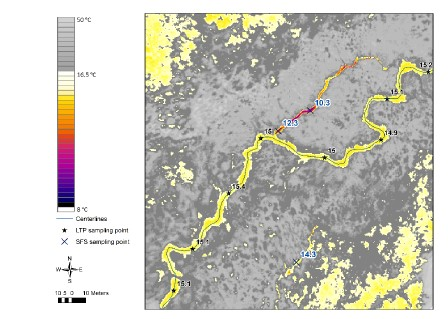
\includegraphics[width=\textwidth,height=3.125in]{./images/example_TIR_figure.jpg}

}

\caption{Example of airborne thermal infrared imagery showing
temperature contrast in a stream. A cold water inflow (purple and blue
colors) enters the main channel (yellow color). Figure from NV5
Geospatial consultants.}

\end{figure}

\hypertarget{from-thermal-infrared-imagery-to-conservation-actions}{%
\section*{From Thermal Infrared Imagery to Conservation
Actions}\label{from-thermal-infrared-imagery-to-conservation-actions}}
\addcontentsline{toc}{section}{From Thermal Infrared Imagery to
Conservation Actions}

\markright{From Thermal Infrared Imagery to Conservation Actions}

Cold Water Refugia, or areas within a stream that are persistently
colder than surrounding areas, are critical features of wild salmon
habitat throughout their range. Stream reaches with cold seeps and
springs often result in much cooler water, which are increasingly
important for wild salmon to keep cool as water temperatures in many
streams have warmed. Some human activities can diminish or extinguish
cold water refugia, such as groundwater withdrawl and construction of
impervious surfaces. To conserve cold water refugia these sites must
first be mapped and identified, and land owners and managers must
understand best practices for their conservation.

Since 2020, three nonprofits - Cook Inletkeeper, Kachemak Heritage Land
trust, and Kenai Watershed Forum - have worked together to identify
where cold water refugia are found in the Kenai Peninsula lowlands, a
region where productive wild salmon habitat intersects with a growing
development footprint. We used cutting-edge methods to locate cold water
refugia with thermal infrared imagery, a technology similar to night
vision goggles that shows heat contrast. Our resulting ``treasure map''
of cold water refugia locations is a valuable tool for prioritizing
conservation and outreach efforts.

In this project we focused our research on tributaries of the Kenai and
Kasilof rivers; specifically in the lower sections of streams outside of
the federally protected Kenai National Wildlife refuge as outlined in
the Mountains to Sea planning document (Morton et al. 2015). Our goals
with this project were:

\begin{enumerate}
\def\labelenumi{\arabic{enumi}.}
\item
  Identify land parcels that contain one or more cold water refugia
  features, and communicate information about these features and
  possible conservation strategies to land owners
\item
  Use a variety of techniques to communicate our results to over sixty
  landowners, agencies, and organizations
\end{enumerate}

Conservation actions that will result from these efforts include parcel
acquisition and conservation easements, voluntary compliance,
stewardship and restoration projects, and voluntary land agreements or
exchanges.

\hypertarget{the-future}{%
\section*{The Future}\label{the-future}}
\addcontentsline{toc}{section}{The Future}

\markright{The Future}

Our efforts in applying thermal imagery data for conservation purposes
highlights the value of recognizing cold water refugia as an asset for
wild salmon habitat (Snyder et al. 2022). The work described here can
continue to expand into additional territiories: there are twenty river
corridors of conservation priority described in the Mountains to Sea
plan, while we possess aerial thermal infrared imagery on just five (the
Anchor river plus the four rivers described in this report) (Mauger,
McCarty, et al. 2015).

Beyond gathering additional thermal infrared imagery data in order for
the work of conserving cold water refugia to have a sustained and
widespread impact beyond this project we recommend that future efforts
develop Alaska-specific technical and legal definitions, and applying
them towards management needs.

Two examples of potential applications follow:

\hypertarget{example-source-water-protection-areas}{%
\subsubsection*{Example: Source Water Protection
Areas}\label{example-source-water-protection-areas}}
\addcontentsline{toc}{subsubsection}{Example: Source Water Protection
Areas}

The U.S. Environmental Protection Agency (U.S. EPA) defines ``Source
Water Protection Areas'' for groundwater sources used for drinking
water, which delineate geographic areas that contribute to the drinking
water supply\footnote{https://www.epa.gov/sourcewaterprotection/delineate-source-water-protection-area}.
Similar logic could apply towards defining the extent of riparian
landscape that supplies cold water refugia. Researchers with Kachemak
Bay National Estuarine Research Reserve (KBNERR) in Homer, Alaska
recently demonstrated that the extent of land that recharges cold water
refugia can be delineated by use of a GIS-based model(Gerlach et al.
2021).

As of winter 2022 the Kenai Peninsula Borough is currently in the
process of reviewing its permitting process for material extraction
sites (i.e.~gravel pits). Initial discussions between the the Borough
and KBNERR have included the possibility of permit reviewers being able
to use their maps of subterranean aquifer flow paths to comment on
proposed development plans. This cooperation could help ensure that
future development minimizes impact on the aquifers that supply cold
water refugia, in the same way that defining Source Water Protection
Areas help protect drinking water sources.

\hypertarget{example-columbia-river-cold-water-refugia}{%
\subsubsection*{Example: Columbia River Cold Water
Refugia}\label{example-columbia-river-cold-water-refugia}}
\addcontentsline{toc}{subsubsection}{Example: Columbia River Cold Water
Refugia}

In an example from the Columbia River in the Pacific Northwest, the U.S.
EPA has taken detailed steps to identify, define, and recommend
conservation actions for cold water refugia. Here, cold water refugia
were defined by quantitative flow volumes and their level of contrast
with connected, warmer water bodies\footnote{https://www.epa.gov/columbiariver/columbia-river-cold-water-refuges-plan}.
Such efforts could set an example for Alaska to follow in beginning to
develop its own technical definitions of cold water refugia.

Existing efforts to technically define cold water refugia have focused
on needs of adult upstream migration. However, salmon at all life stages
benefit from a mosaic of water temperature environments, such as when
juvenile fry migrate between colder and warmer and areas to feed and
digest (Armstrong et al. 2013). Thus it is recommended that future
technical definitions also consider the needs of juvenile salmon.

\hypertarget{next-steps}{%
\section*{Next Steps}\label{next-steps}}
\addcontentsline{toc}{section}{Next Steps}

\markright{Next Steps}

We will continue to use our existing dataset to prioritize land
conservation efforts in the Kenai Peninsula lowlands area. Currently we
have surveyed the lower sections of four tributaries, while the
Mountains to Sea document highlights twenty priority river corridors as
conservation targets.

Specific actions that will continue to support the goals of this project
include:

\begin{itemize}
\item
  Identifying where current, future, and retired material extraction
  sites (i.e.~gravel pits) may influence conservation goals in the 20
  Mountains to Stream corridors, and supporting efforts to include
  groundwater considerations in permit reviews
\item
  Continue to communicate with the local U.S. Fish and Wildlife office,
  which in 2022 initiated an effort to gather aerial thermal infrared
  imagery in local river corridors used by migrating adult coho
  salmon\footnote{https://www.peninsulaclarion.com/sports/refuge-notebook-flying-a-remote-sensing-mission-on-the-refuge/}.
  A cost-effective collaboration could result if USFWS aerial thermal
  imagery can be used for the same conservation goals as detailed in
  this project
\item
  Continue to communicate with the Alaska Department of Environmental
  Conservation and other agencies about moving towards formally defined
  standards for cold water refugia
\item
  Develop and publish standards for collection and application of
  thermal imagery in aquatic habitat, similar to published standards for
  stream temperature monitoring (Mauger, Shaftel, et al. 2015a)
\item
  Convert the thermal imagery map files acquired from this project to a
  format accessible from an online web browser or Google Earth
\end{itemize}

A two-page project summary titled, ``Science Based Land Conservation:
Cold Water Stepping Stones'' is outlined below in
Figure~\ref{fig-summary-sheet}. Download a full size version of this
information by clicking on the link below.

\begin{figure}

{\centering 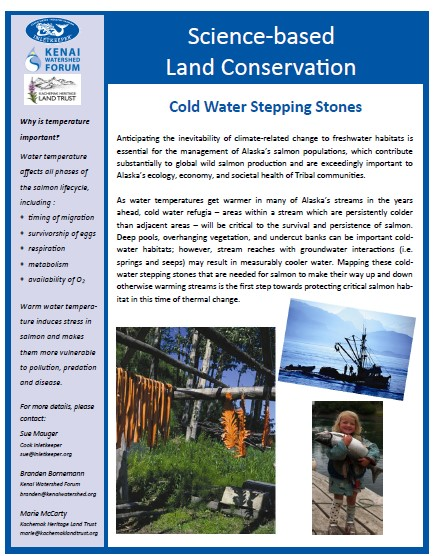
\includegraphics[width=4.16667in,height=5.20833in]{./images/project_summary_img.jpg}

}

\caption{\label{fig-summary-sheet}Project Summary Sheet}

\end{figure}

\bookmarksetup{startatroot}

\hypertarget{introduction}{%
\chapter{Introduction}\label{introduction}}

The following chapters contain data and analysis related to the Kenai
River Thermal Imagery project conducted from 2020 - 2022. This work is a
collaborative effort between three Kenai Peninsula Nonprofits: Cook
Inletkeeper, Kachemak Bay Heritage Land Trust, and Kenai Watershed
Forum. It is funded by the Alaska Sustainable Salmon Fund (project
\#53003).

This report is generated using Quarto, an open source publishing
platform. It is best accessed online at the url
\url{https://kenaiwatershed.quarto.pub/kenai_thermal_imagery/}.

All code used to generate this report is available in the project's
GitHub repository at
\url{https://github.com/Kenai-Watershed-Forum/kenai_thermal_imagery_v2}.

\bookmarksetup{startatroot}

\hypertarget{project-map}{%
\chapter{Project Map}\label{project-map}}

Our research focused on four streams in the Kenai Peninsula lowlands
region in southcentral Alaska:

\begin{itemize}
\item
  Three tributaries of the lower Kenai River

  \begin{itemize}
  \item
    Moose River
  \item
    Beaver Creek
  \item
    Funny River
  \end{itemize}
\item
  One tributary of the lower Kasilof River

  \begin{itemize}
  \tightlist
  \item
    Crooked Creek
  \end{itemize}
\end{itemize}

The ArcGIS Online project map may be accessed below or at
\href{https://arcg.is/0vaueq}{ArcGIS Online (Click Here:
https://arcg.is/0vaueq)}.

The online map contains layers with the following data:

\begin{itemize}
\item
  Project Watershed Boundaries
\item
  National Hydrography Database (rivers, lakes, streams, etc)
\item
  Anadromous Waters Catalog

  \begin{itemize}
  \item
    Streams
  \item
    Lakes
  \end{itemize}
\item
  Kenai Peninsula Borough Parcel Boundaries
\item
  Thermal Imagery Data from NV5 Geospatial consultants report

  \begin{itemize}
  \item
    Significant Thermal Features (identified from thermal imagery)
  \item
    Longitudinal Temperature Profiles (main channel temperatures of
    study streams)
  \item
    Water Temperature Logger Sites
  \end{itemize}
\end{itemize}

\bookmarksetup{startatroot}

\hypertarget{thermal-imagery-data}{%
\chapter{Thermal Imagery Data}\label{thermal-imagery-data}}

To acquire and prepare thermal aerial infrared imagery, we worked with
\href{https://www.nv5.com/geospatial/}{NV5 Geospatial}\footnote{https://www.nv5.com/geospatial/}
(formerly Watershed Sciences, Inc), a contractor who has led prior
efforts in the region to gather thermal aerial infrared data for aquatic
habitat research (Watershed Sciences 2010). On July 5, 2020, NV5
collected thermal infrared imagery from a helicopter-mounted camera for
the four steams on the Kenai Peninsula lowlands that were the focus of
this study (Beaver Creek, Funny River, Moose River, and Crooked Creek).
All streams were flown during the afternoon hours in order to maximize
the thermal contrast between the river's water and the banks.

The surveys extend for a total length of 59.1 km of the streams. Flight
transects proceeded from the mouth of each stream in an upstream
direction. The data were collected to aid the team in identifying the
spatial variability in surface temperatures as well as thermal influence
of point sources, tributaries, and surface springs.

Specific deliverables generated by NV5 Geospatial from the thermal
imagery data include:

\begin{itemize}
\item
  Rasters (map image files; .tif and .jpg formats)
\item
  Shapefiles (longitudinal temperature profiles, stream centerlines,
  others; .shp format)
\item
  Other supplemental items (coordinates of significant thermal features,
  maps and figures, and others)
\end{itemize}

The full technical report from NV5 Geospatial describing detailed
methods and interpretation can be downloaded at the following link in
the online version of this report:

The image raster files are of a large size (\textasciitilde3 GB) and may
be acquired by contacting staff at Cook Inletkeeper
(sue@inletkeeper.org), Kenai Watershed Forum
(hydrology@kenaiwatershed.org), or Kachemak Heritage Land Trust
(info@kachemaklandtrust.org).

\hypertarget{parcel-data-summary}{%
\section{Parcel data summary}\label{parcel-data-summary}}

We generated a table in GIS (ArcMap Pro 10.8.1) of parcels in the Kenai
Peninsula Borough that intersect with cold-water inputs (e.g.~seeps,
springs) within the surveyed areas of Beaver Creek, Crooked Creek, Moose
River, and Funny River. We identified a total of n = 31 unique parcels
containing a total of n = 63 unique cold water refugia features.

\textbf{?@fig-parcel-plot} summarizes the ownership type of these
parcels by general category of owner type.

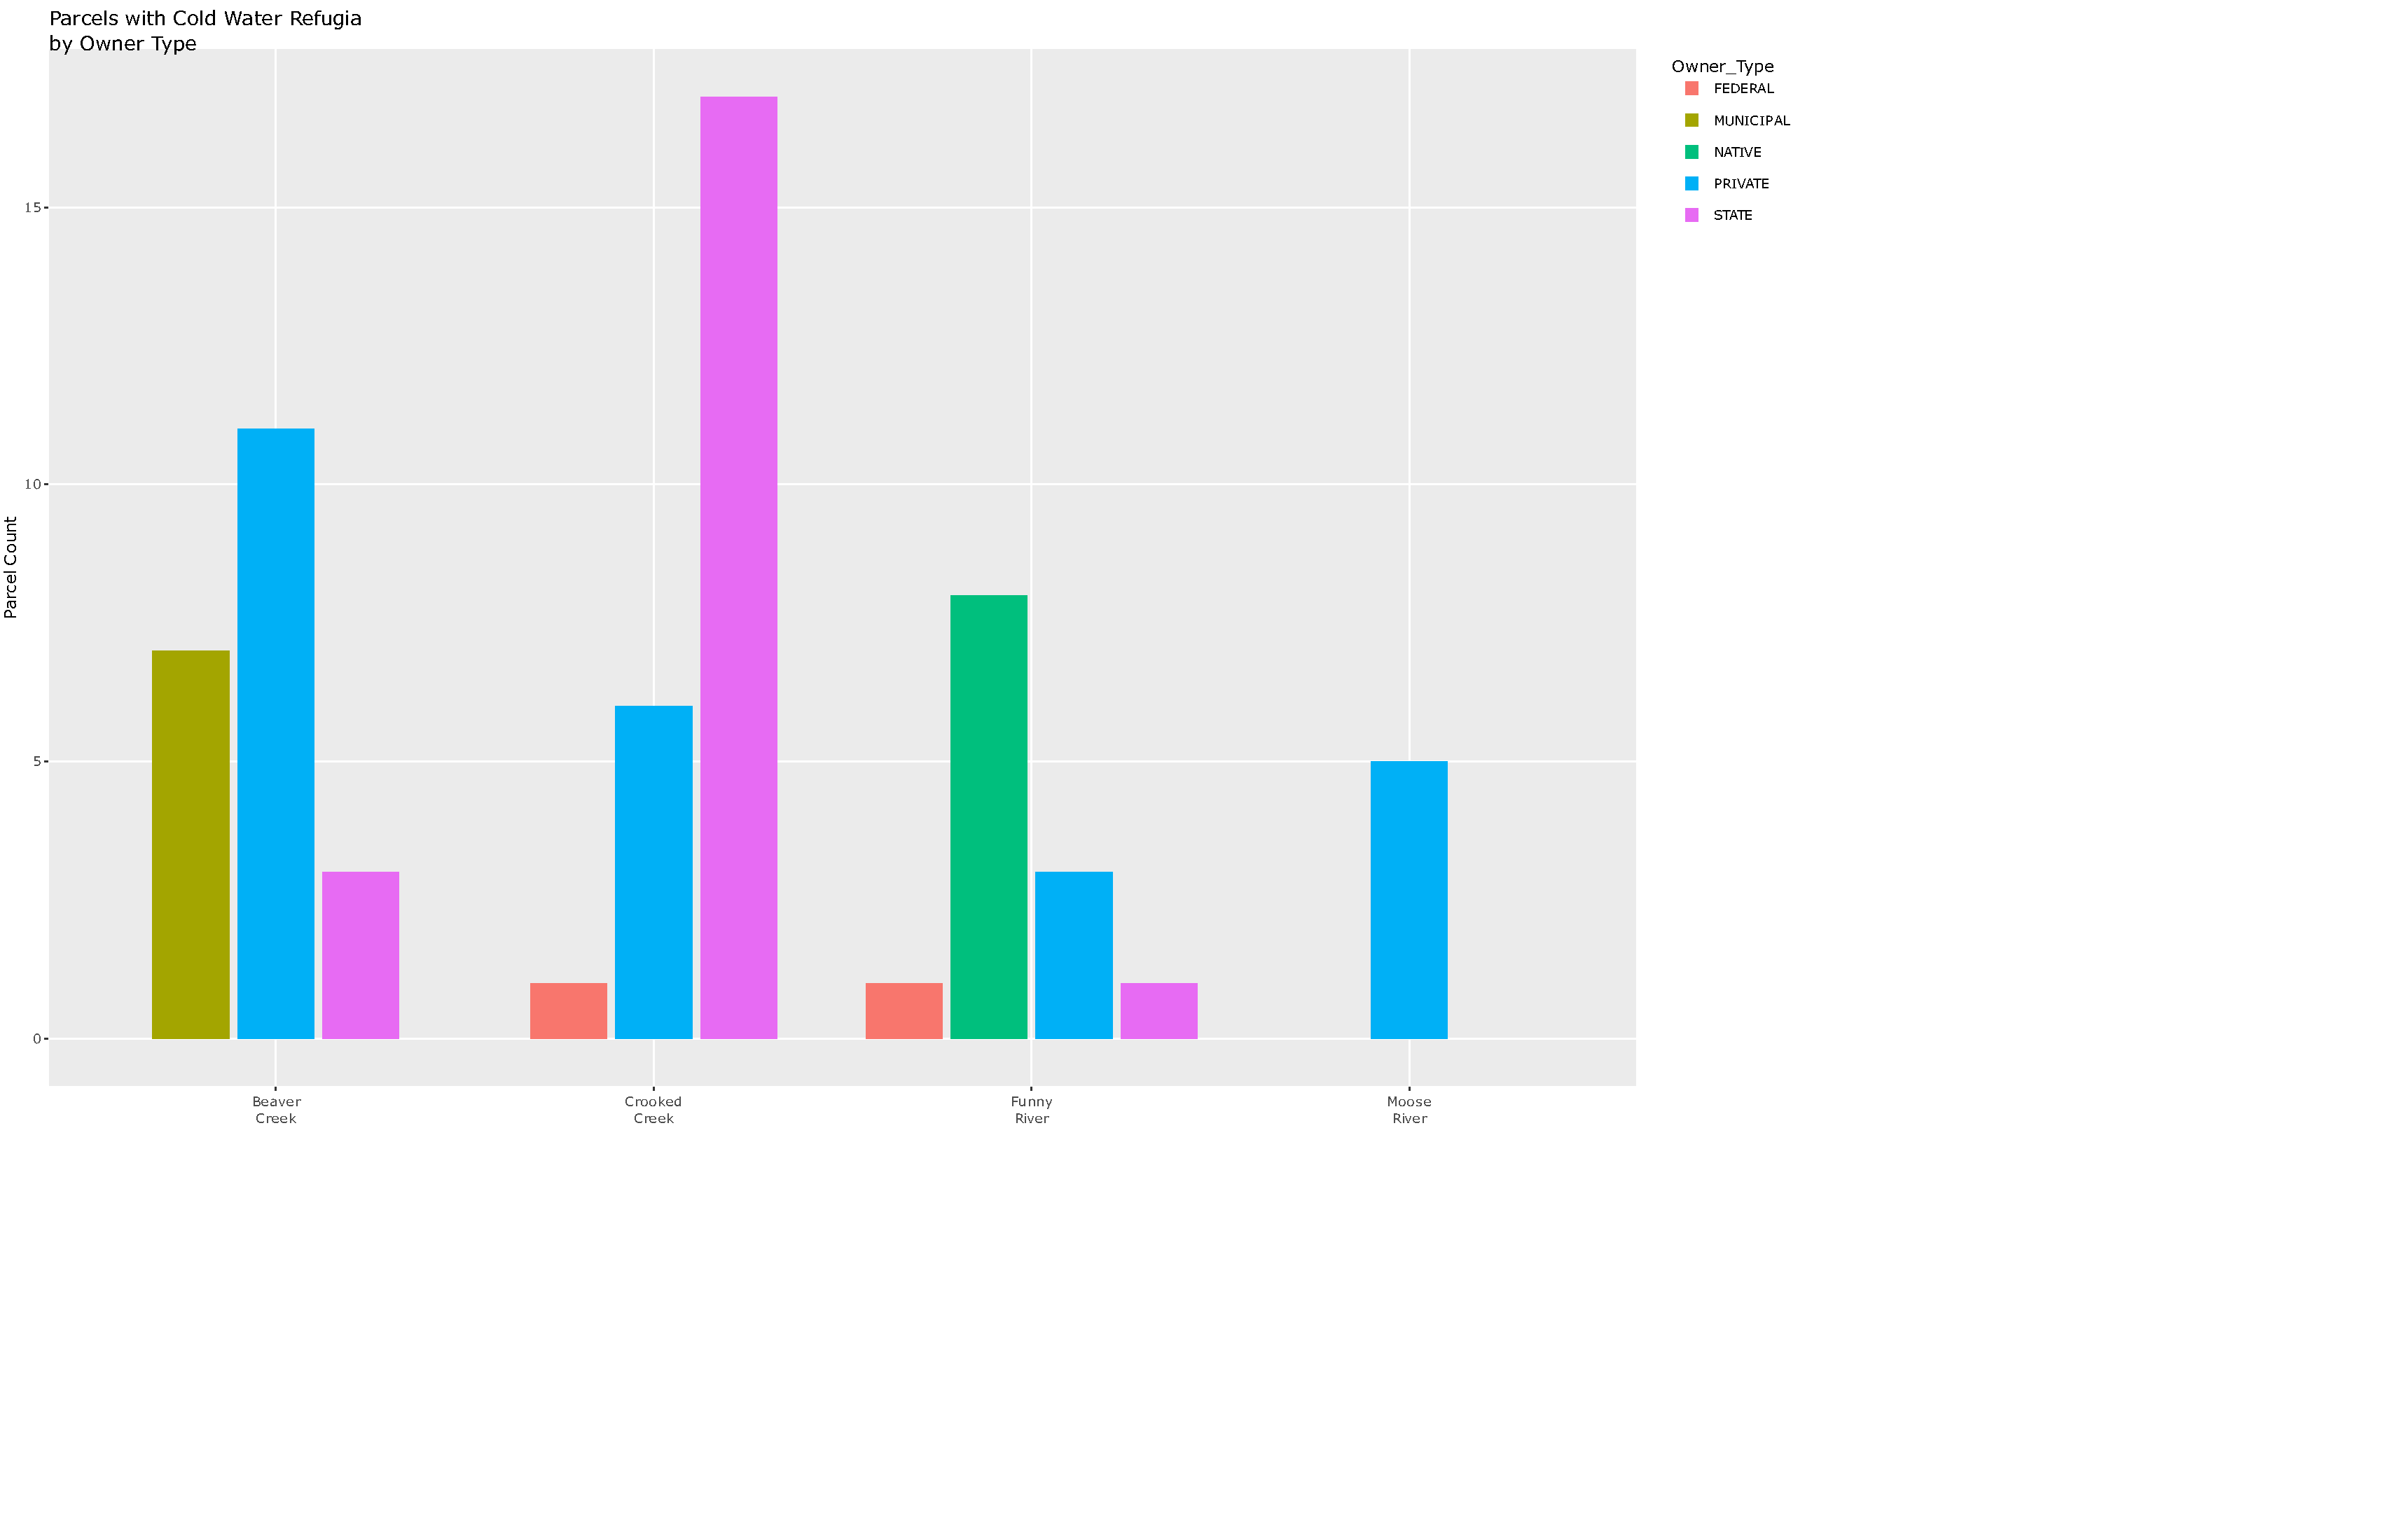
\includegraphics{./thermal_imagery_data_files/figure-pdf/parcel-plot-1.pdf}

\hypertarget{ground-truth-data}{%
\section{Ground truth data}\label{ground-truth-data}}

On July 7-8, 2021 we visited a subset of sites identified by the NV5
Geospatial Consultants report as cold water features. We visited 12 of
63 total sites. We recorded surface water temperatures of the identified
features as well as the adjacent main stem using a using a Hach Sension
5 portable meter. The average time difference between main stem
temperature observation and off-channel observation was 13.9 minutes. We
created a graphic sketch of the layout of each feature, and recorded
site photos.

Field forms, including site sketches, can be accessed at the following
link:

In general we observed symmetry in the pattern of temperature contrast
for both our ground-truthed data as well as temperatures observed from
the thermal aerial infrared dataset. This indicates that the temperature
contrasts identified from the aerial imagery are persistent and not
ephemeral. Figure~\ref{fig-gt-tir-obs-beaver} through
Figure~\ref{fig-gt-tir-obs-funny} visualize water temperature data
sourced from the significant features in aerial imagery on July 20, 2020
along with ground-truthed measurements from July 7-8, 2021.

Note that the temperature data reported from thermal infrared imagery
observations consists of multiple statistics, whereas the ground-truth
values consist of a single observation. Multiple statistics are reported
for the aerial thermal infrared temperature values as a result of the
sampling method used, wherein ten surface temperatures within a
two-meter radius are evaluated. See the, ``Interpretation and Sampling''
section in the technical report from NV5 Geospatial Consultants,
available for download above (NV5 Geospatial 2021).

\begin{figure}

{\centering 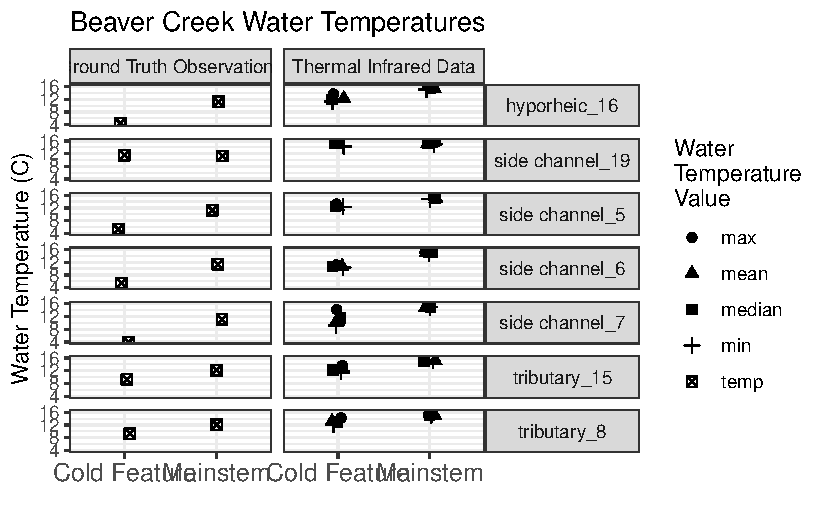
\includegraphics{./thermal_imagery_data_files/figure-pdf/fig-gt-tir-obs-beaver-1.pdf}

}

\caption{\label{fig-gt-tir-obs-beaver}Beaver Creek water temperatures,
ground truth and thermal infrared imagery observations.}

\end{figure}

\begin{figure}

{\centering 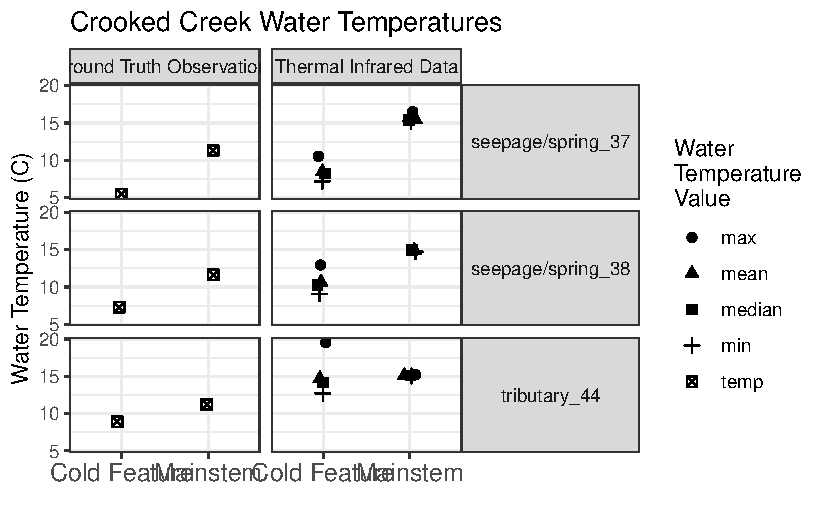
\includegraphics{./thermal_imagery_data_files/figure-pdf/fig-gt-tir-obs-crooked-1.pdf}

}

\caption{\label{fig-gt-tir-obs-crooked}Crooked Creek water temperatures,
ground truth and thermal infrared imagery observations.}

\end{figure}

\begin{figure}

{\centering 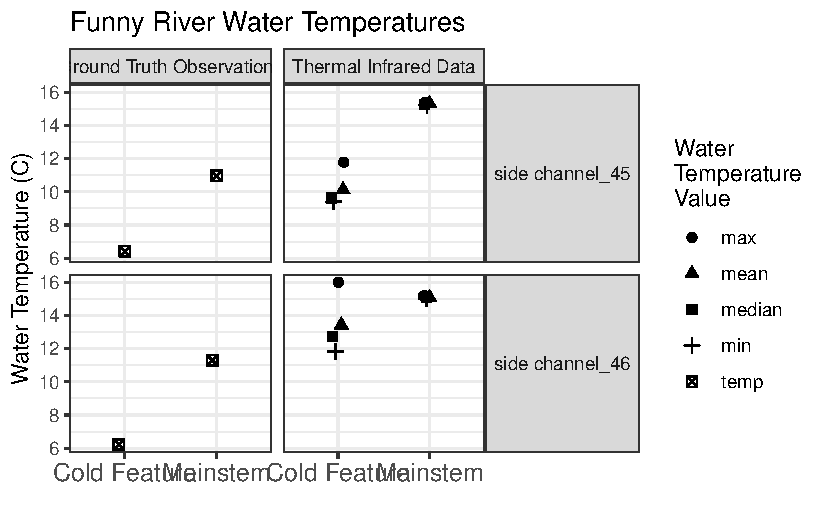
\includegraphics{./thermal_imagery_data_files/figure-pdf/fig-gt-tir-obs-funny-1.pdf}

}

\caption{\label{fig-gt-tir-obs-funny}Funny River water temperatures,
ground truth and thermal infrared imagery observations.}

\end{figure}

\hypertarget{collaborative-assessment}{%
\section{Collaborative Assessment}\label{collaborative-assessment}}

Researchers with participating organizations assessed conservation
strategies within each study watershed, and recorded their notes on a
shared platform. These collective notes are being used internally to
inform strategy for outreach approaches with local property owners.

Data sources used to assess parcel-specific conservation strategies
include:

\begin{itemize}
\item
  Custom maps for each significant thermal feature, including
  information about the parcel or parcels that it occupies
\item
  Information about individual thermal features from the
  \href{https://github.com/Kenai-Watershed-Forum/kenai_thermal_imagery/blob/master/documents/TIR_Technical_Data_Report_Kenai_Rivers_20210107.pdf}{NV5
  Geospatial Consultants Report}, including mean value and contrast with
  the main stem
\item
  The \href{https://arcg.is/fzn14}{ArcGIS Online project map}
\end{itemize}

\textbf{Project collaborators may access the Thermal Imagery Database
Google Sheet using the link below:}

\textbf{Link:
\href{https://docs.google.com/document/d/1TZcTMBOL6WDCyvOODZlGeuCd-1sPWzYsurWtx7MJoUE/edit}{Thermal
Imagery Collaborative Assessment}}

An example map is shown in Figure 3.5.

\begin{figure}

{\centering 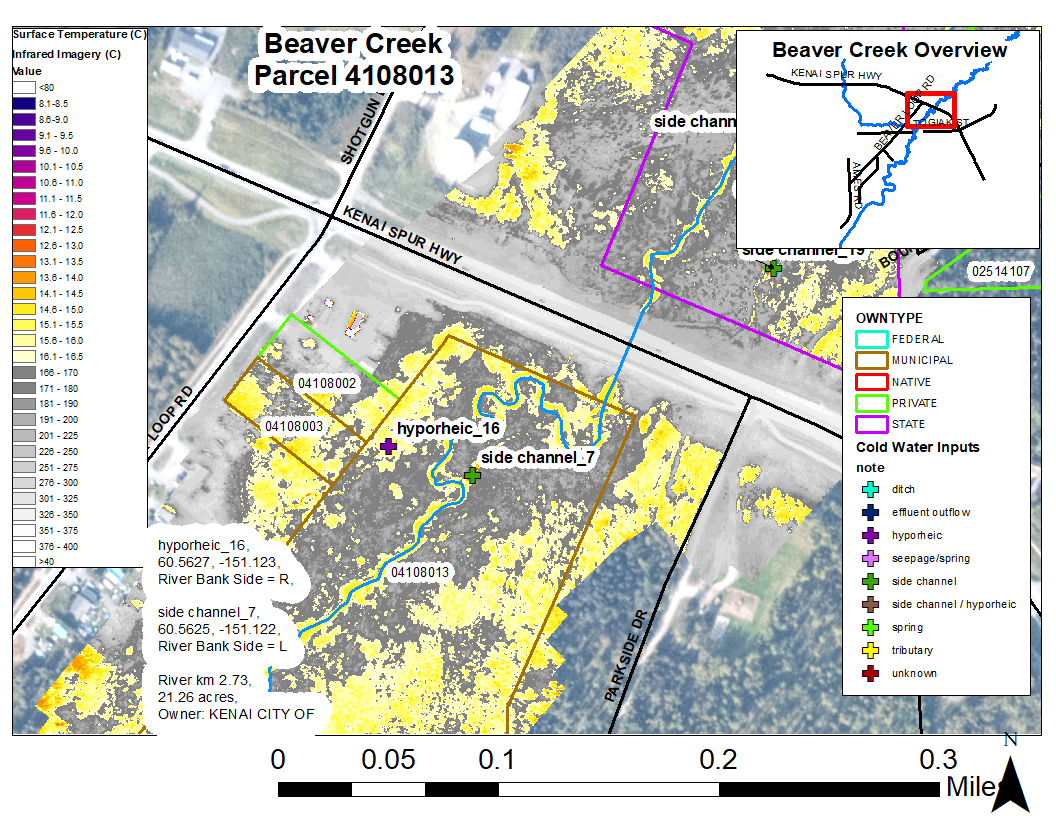
\includegraphics[width=3.90625in,height=3.38542in]{./images/Beaver_Crk4.png}

}

\caption{\label{fig-example-map}Example of airborne thermal infrared
imagery map with parcel overlay.}

\end{figure}

\bookmarksetup{startatroot}

\hypertarget{water-temperature-loggers}{%
\chapter{Water Temperature Loggers}\label{water-temperature-loggers}}

In order to supplement aerial thermal infrared imagery and cold-feature
ground truthing data, we deployed water temperature loggers in the lower
reach of each study stream to collect continuous time series of water
temperature. We used Onset HOBO Temp Pro V2 loggers, deployed and
maintained according to published regional standards (Mauger, Shaftel,
et al. 2015b).

This section describes methods to visualize and perform basic quality
checks on continuous temperature loggers deployed in the study streams.
All data files (.csv) used in these analyses can be downloaded from this
project's
\href{https://github.com/Kenai-Watershed-Forum/kenai_thermal_imagery/tree/master/input}{GitHub
repository}.

\hypertarget{locations}{%
\section{Locations}\label{locations}}

See the Project Map (Section 2) section of this report for locations of
water temperature logger sites. The ArcGIS Online layer titled, ``Water
Temperature Logger Sites'' displays these locations.

Locations will also be reflected in the Alaska Center for Conservation
Science's AKOATS map
(\href{https://accs.uaa.alaska.edu/aquatic-ecology/akoats/}{Alaska
Online Aquatic Temperature Site})\footnote{https://accs.uaa.alaska.edu/aquatic-ecology/akoats/}
in Spring 2023.

\hypertarget{additional-data-preparation}{%
\section{Additional Data
Preparation}\label{additional-data-preparation}}

Some water temperature time series downloaded from loggers required
additional examination in order to prepare them for submission to
AKOATS. See Appendix A, Temperature Logger Data Preparation for
additional details.

\newpage

\bookmarksetup{startatroot}

\hypertarget{applications}{%
\chapter{Applications}\label{applications}}

We applied our findings of where cold-water inputs were located towards
education and outreach opportunities in the Central Kenai Peninsula
region. We used a variety of methods including comments on public land
management plans, direct mailers, cooperative planning with peer
researchers, and communication with state and federal agency staff.

We used the thermal features map layer generated from this project as a
tool to help generate comments on a local land management plan. We
commented on the
\href{https://www.kenai.city/lands/page/land-management-plan}{City of
Kenai 2021 Land Management Plan}, which highlighted a number of parcels
in the Beaver Creek corridor, and recommended parcel-specific actions
(e.g.~retain, sell, re-zone).

We created a separate map showing parcels highlighted in the plan, with
management status available in a point and click format. The parcels
were superimposed on a several layers highlighting ecological values
such as wetlands and anadromous streams, as well as the thermal features
identified in this project. Methods are described in a separate
stand-alone document at \url{https://rpubs.com/kwf/867931}.

Access the City of Kenai Land Management Plan Comments Map here:
\url{https://arcg.is/1Oq9Kq}.

Access PDFs of submitted Public Comments below:

\hypertarget{landowner-outreach}{%
\section{Landowner Outreach}\label{landowner-outreach}}

\hypertarget{letter}{%
\subsection{Letter}\label{letter}}

We composed a letter addressed to landowners whose property contains
cold water features that flow in to one of our study streams. This
letter describes the nature of the project and the value of cold water
features to salmon habitat. Landowners are invited to contact the
researchers if they would like more information about their specific
property.

A draft version of the letter to landowners may be accessed below:

\hypertarget{postcard}{%
\subsection{Postcard}\label{postcard}}

We designed and mailed a post card to landowners whose property contains
cold water features that flow in to one of our study streams. The
postcard notifies landowners that their specific parcels are of high
conservation value, and encourages them contact project scientists to
learn more about best practices.

A PDF proof version of the postcard may be accessed below:

\hypertarget{communication-with-local-state-and-federal-agency-staff}{%
\subsection{Communication with local State and Federal Agency
Staff}\label{communication-with-local-state-and-federal-agency-staff}}

We met with state and federal agency staff to discuss the nature of our
research and its applications.

\begin{itemize}
\item
  In conversations with staff from the Alaska Department of
  Environmental Conservation (ADEC), we learned more about the process
  by which new research such as ours may be applied in the future.
  Emerging research on how water quality issues may affect freshwater
  fish habitat is typically first evaluated by the Alaska Department of
  Fish and Game (ADF\&G) before being evaluated in a regulatory context
  such as ADEC. With that in mind, our final reports will be made
  available to ADF\&G staff.
\item
  On June 1, 2022 we met with local U.S. Fish and Wildlife staff to
  discuss the nature of thermal infrared imagery gathered in summer 2022
  for a separate USFWS project related to adult coho salmon movement.
  These data are currently being evaluated, and it is our hope that they
  may later also be applicable for the purposes of identify cold water
  refugia in the conservation priority corridors identified in the
  Mountains to Sea report (Morton et al. 2015)
\end{itemize}

\hypertarget{local-interest-in-conservation-easement}{%
\subsection{Local interest in Conservation
Easement}\label{local-interest-in-conservation-easement}}

We also communicated with the Snowshoe Gun Club, one of the larger
private landowners in the lower Beaver Creek corridor. The gun club's
ground footprint currently is set back several hundred yards from
adjacent riparian zones and can be considered compatible with fish
habitat management.

The Club has expressed interest in developing conservation easement
status for part of their current land holdings, along with an adjacent
parcel also set on Beaver Creek also currently in private ownership. We
provided a custom map (Figure~\ref{fig-sgc-map}) to highlight cold water
refugia features on these parcels, available for download below.
Discussions will continue with the Club to determine interest in moving
forward with a potential conservation easement.

\begin{figure}

{\centering 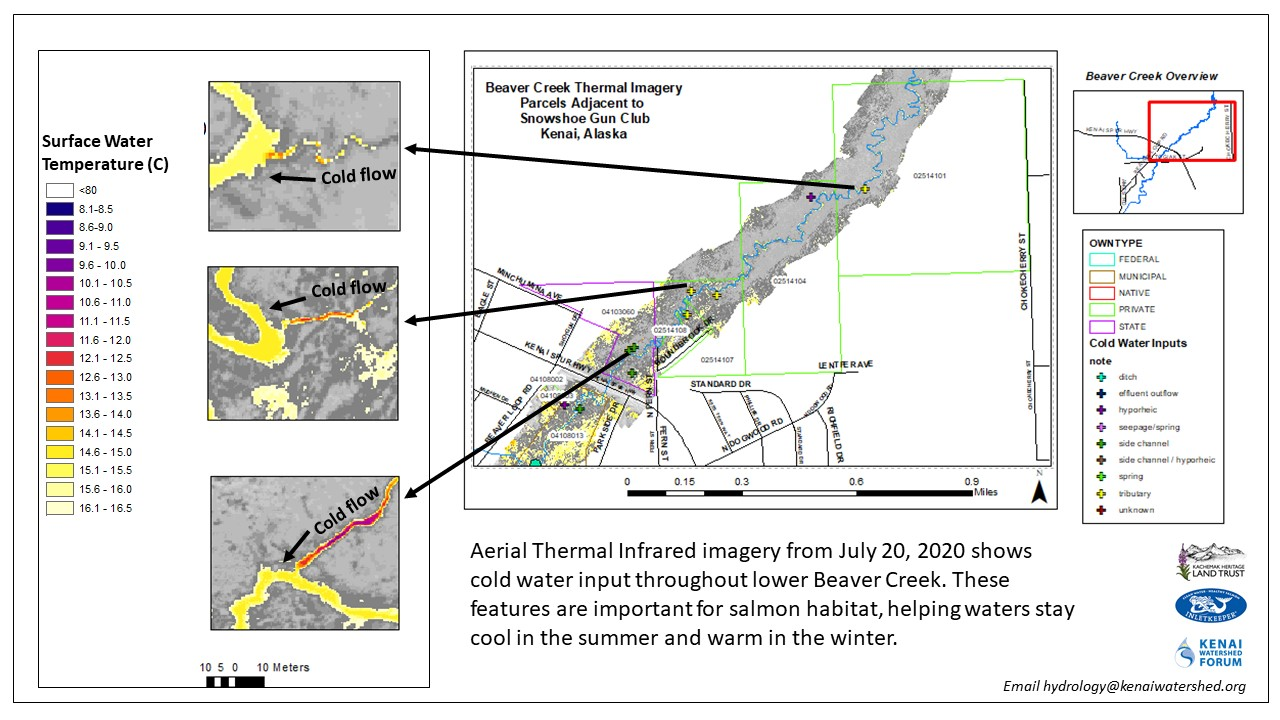
\includegraphics[width=\textwidth,height=4.16667in]{./images/Snowshoe_Gun_Club_Thermal_Imagery_map.jpg}

}

\caption{\label{fig-sgc-map}Cold water refugia site highlights near
Snowshoe Gun Club}

\end{figure}

\bookmarksetup{startatroot}

\hypertarget{summary}{%
\chapter{Summary}\label{summary}}

The following are general observations regarding conservation potential
for each of the stream corridors in this study. The stream distance and
property ownership information cited is from (Morton et al. 2015). For
more details on land ownership and watershed-specific conservation
opportunities, see the Mountains to Sea report.

\hypertarget{general-recommendations-by-stream-corridor}{%
\section{General Recommendations by Stream
Corridor}\label{general-recommendations-by-stream-corridor}}

\begin{verbatim}
-- Attaching packages --------------------------------------- tidyverse 1.3.2 --
v ggplot2 3.4.0      v purrr   1.0.0 
v tibble  3.1.8      v dplyr   1.0.10
v tidyr   1.2.1      v stringr 1.5.0 
v readr   2.1.3      v forcats 0.5.2 
-- Conflicts ------------------------------------------ tidyverse_conflicts() --
x dplyr::filter() masks stats::filter()
x dplyr::lag()    masks stats::lag()
\end{verbatim}

\hypertarget{beaver-creek}{%
\subsection{Beaver Creek}\label{beaver-creek}}

Beaver Creek runs a total of 21.8 river miles before meeting the Kenai
River, with 4.0 of those miles in the lower section outside the Kenai
National Wildlife Refuge.

Land ownership in the lower Beaver Creek corridor can be described as
very parcelized, with the majority of parcels that are directly adjacent
to the creek in private ownership (20 of 28), most of them accessible
via Beaver Loop road. In our work, we found that 21 of these parcels
contained cold water refugia features (Figure 3.1).

In the context of near-term potential conservation opportunities,
several categories are highlighted. Several parcels belonging to the
City of Kenai are recommended in the 2021 Land Management Plan for
rezoning to recognize their conservation value. Our submitted comments
support this goal. Additionally, the 160 acre parcel that Snowshoe Gun
Club is considering for conservation easement status also stands out. We
intend to continue the dialogue with the club to ensure that the
opportunity for potential easement status can be easily accessed when
they choose to proceed.

\hypertarget{funny-river}{%
\subsection{Funny River}\label{funny-river}}

Funny River runs a total of 67 river miles before meeting the Kenai
River, with 4.5 of those miles in the lower section outside the Kenai
National Wildlife Refuge.

The lower Funny River riparian corridor can be described as primarily
under ownership of private individuals, the Alaska Department of Natural
Resources (AKDNR), and the regional native corporation CIRI (Cook Inlet
Regional Incorporated).

In the context of near-term potential for conservation opportunities,
several categories are highlighted. An AKDNR parcel that parallels Funny
River Road contains a significant cold water feature that we visited on
foot ground truth. Future road improvement projects would ideally be
cognizant of such features and take efforts to minimize impact from
impervious surfaces.

An additional parcel owned by CIRI approximately 4 miles upstream
contains a cluster of six cold-water features. This parcel also contains
tributaries not currently documented as anadromous but very likely are.
We intend to communicate the conservation values of this parcel to CIRI
so that they may be best informed for future land management decisions.

\hypertarget{moose-river}{%
\subsection{Moose River}\label{moose-river}}

Funny River runs a total of 137 river miles before meeting the Kenai
River, with 2.2 of those miles in the lower section outside the Kenai
National Wildlife Refuge.

We identified a minimal number of cool-water refugia features in the
lower Moose River. All of these features lie on privately owned parcels.
In our efforts to contact Moose River landowners to share educational
materials we failed to receive responses.

At current time, we intend to continue seeking opportunities to
communicate with Moose River landowners. Future community opportunities
and events will likely present new opportunties to share our findings
with specific landowners.

\hypertarget{crooked-creek}{%
\subsection{Crooked Creek}\label{crooked-creek}}

Crooked Creek runs a total of 45.9 river miles before meeting the
Kasilof River, with 16.8 of those miles in the lower section outside the
Kenai National Wildlife Refuge.

In the context of near-term potential for conservation opportunities,
several categories are highlighted. The majority of cold-water features
(17/25) lie on state-owned land, and are generally clustered together in
close groups.

An AKDNR parcel that parallels the Sterling Highway and adjacent
subdivisions contains several significant cold water features that we
visited on foot ground truth. Future road and home improvement projects
would ideally be cognizant of such features and take efforts to minimize
impact from impervious surfaces. We recommend a follow-up meeting with
AKDNR officials to highlight these results.

\bookmarksetup{startatroot}

\hypertarget{references}{%
\chapter*{References}\label{references}}
\addcontentsline{toc}{chapter}{References}

\markboth{References}{References}

\hypertarget{refs}{}
\begin{CSLReferences}{1}{0}
\leavevmode\vadjust pre{\hypertarget{ref-armstrong2013}{}}%
Armstrong, Jonathan B., Daniel E. Schindler, Casey P. Ruff, Gabriel T.
Brooks, Kale E. Bentley, and Christian E. Torgersen. 2013. {``Diel
Horizontal Migration in Streams: Juvenile Fish Exploit Spatial
Heterogeneity in Thermal and Trophic Resources.''} \emph{Ecology} 94
(9): 2066--75. \url{https://doi.org/10.1890/12-1200.1}.

\leavevmode\vadjust pre{\hypertarget{ref-gerlach2021}{}}%
Gerlach, Mary E., Kai C. Rains, Edgar J. Guerrón-Orejuela, William J.
Kleindl, Joni Downs, Shawn M. Landry, and Mark C. Rains. 2021. {``Using
Remote Sensing and Machine Learning to Locate Groundwater Discharge to
Salmon-Bearing Streams.''} \emph{Remote Sensing} 14 (1): 63.
\url{https://doi.org/10.3390/rs14010063}.

\leavevmode\vadjust pre{\hypertarget{ref-mauger2015b}{}}%
Mauger, Sue, Marie McCarty, Mandy Bernard, and Branden Bornemann. 2015.
{``Science-Based Land Conservation: Conservation Strategies to Protect
Key Salmon Habitat in Lower Kenai Peninsula Watersheds.''}
\url{https://inletkeeper.org/wp-content/uploads/2017/10/Science-based-Land-Conservation-report.pdf}.

\leavevmode\vadjust pre{\hypertarget{ref-mauger2015}{}}%
Mauger, Sue, Rebecca Shaftel, E. Jamie Trammell, Marcus Geist, and Dan
Bogan. 2015a. {``Stream Temperature Data Collection Standards for
Alaska: Minimum Standards to Generate Data Useful for Regional-Scale
Analyses.''} \emph{Journal of Hydrology: Regional Studies} 4
(September): 431--38. \url{https://doi.org/10.1016/j.ejrh.2015.07.008}.

\leavevmode\vadjust pre{\hypertarget{ref-mauger2015a}{}}%
---------. 2015b. {``Stream Temperature Data Collection Standards for
Alaska: Minimum Standards to Generate Data Useful for Regional-Scale
Analyses.''} \emph{Journal of Hydrology: Regional Studies} 4
(September): 431--38. \url{https://doi.org/10.1016/j.ejrh.2015.07.008}.

\leavevmode\vadjust pre{\hypertarget{ref-morton2015}{}}%
Morton, J M, D R Magness, M McCarty, D Wigglesworth, R Ruffner, M
Bernard, N Walker, et al. 2015. {``Kenai Mountains to Sea: A Land
Conservation Strategy to Sustain Our Way of Life on the Kenai
Peninsula.''}
\url{https://kenaiwatershed.org/wp-content/uploads/2019/03/Kenai-Mountains-to-Sea-Strategic-Plan_5nov2016_compressed.pdf}.

\leavevmode\vadjust pre{\hypertarget{ref-nv5geospatial2021}{}}%
NV5 Geospatial. 2021. {``Kenai Rivers - Thermal Infrared Airborne
Imagery Technical Data Report.''} Homer, Alaska.

\leavevmode\vadjust pre{\hypertarget{ref-snyder2022}{}}%
Snyder, Marcía N., Nathan H. Schumaker, Jason B. Dunham, Joseph L.
Ebersole, Matthew L. Keefer, Jonathan Halama, Randy L. Comeleo, et al.
2022. {``Tough Places and Safe Spaces: Can Refuges Save Salmon from a
Warming Climate?''} \emph{Ecosphere} 13 (11).
\url{https://doi.org/10.1002/ecs2.4265}.

\leavevmode\vadjust pre{\hypertarget{ref-watershedsciences2010}{}}%
Watershed Sciences. 2010. {``Airborne Thermal Infrared Remote Sensing:
Anchor River Basin, Alaska.''} Homer, Alaska.
\url{https://inletkeeper.org/wp-content/uploads/2017/10/Airborne-Thermal-Infrared-Remote-Sensing-Anchor-River-Basin-Alaska.pdf}.

\end{CSLReferences}

\appendix
\addcontentsline{toc}{part}{Appendices}

\hypertarget{temperature-logger-data-preparation}{%
\chapter{Temperature Logger Data
Preparation}\label{temperature-logger-data-preparation}}

\hypertarget{water-temperature-logger-data-qaqc}{%
\section{Water Temperature Logger Data
QA/QC}\label{water-temperature-logger-data-qaqc}}

Water temperarture data retrieved from the field was subjected to a
basic quality assurance process before being incorporated into the
analysis dataset. We visually inspected each water temperature time
series and excluded data indicative of pre/post deployment or exposure.
Figure~\ref{fig-preqa} and Figure~\ref{fig-postqa} provide a visual
example of water temperature time series prior to and post quality
assurance processes.

\begin{figure}

{\centering 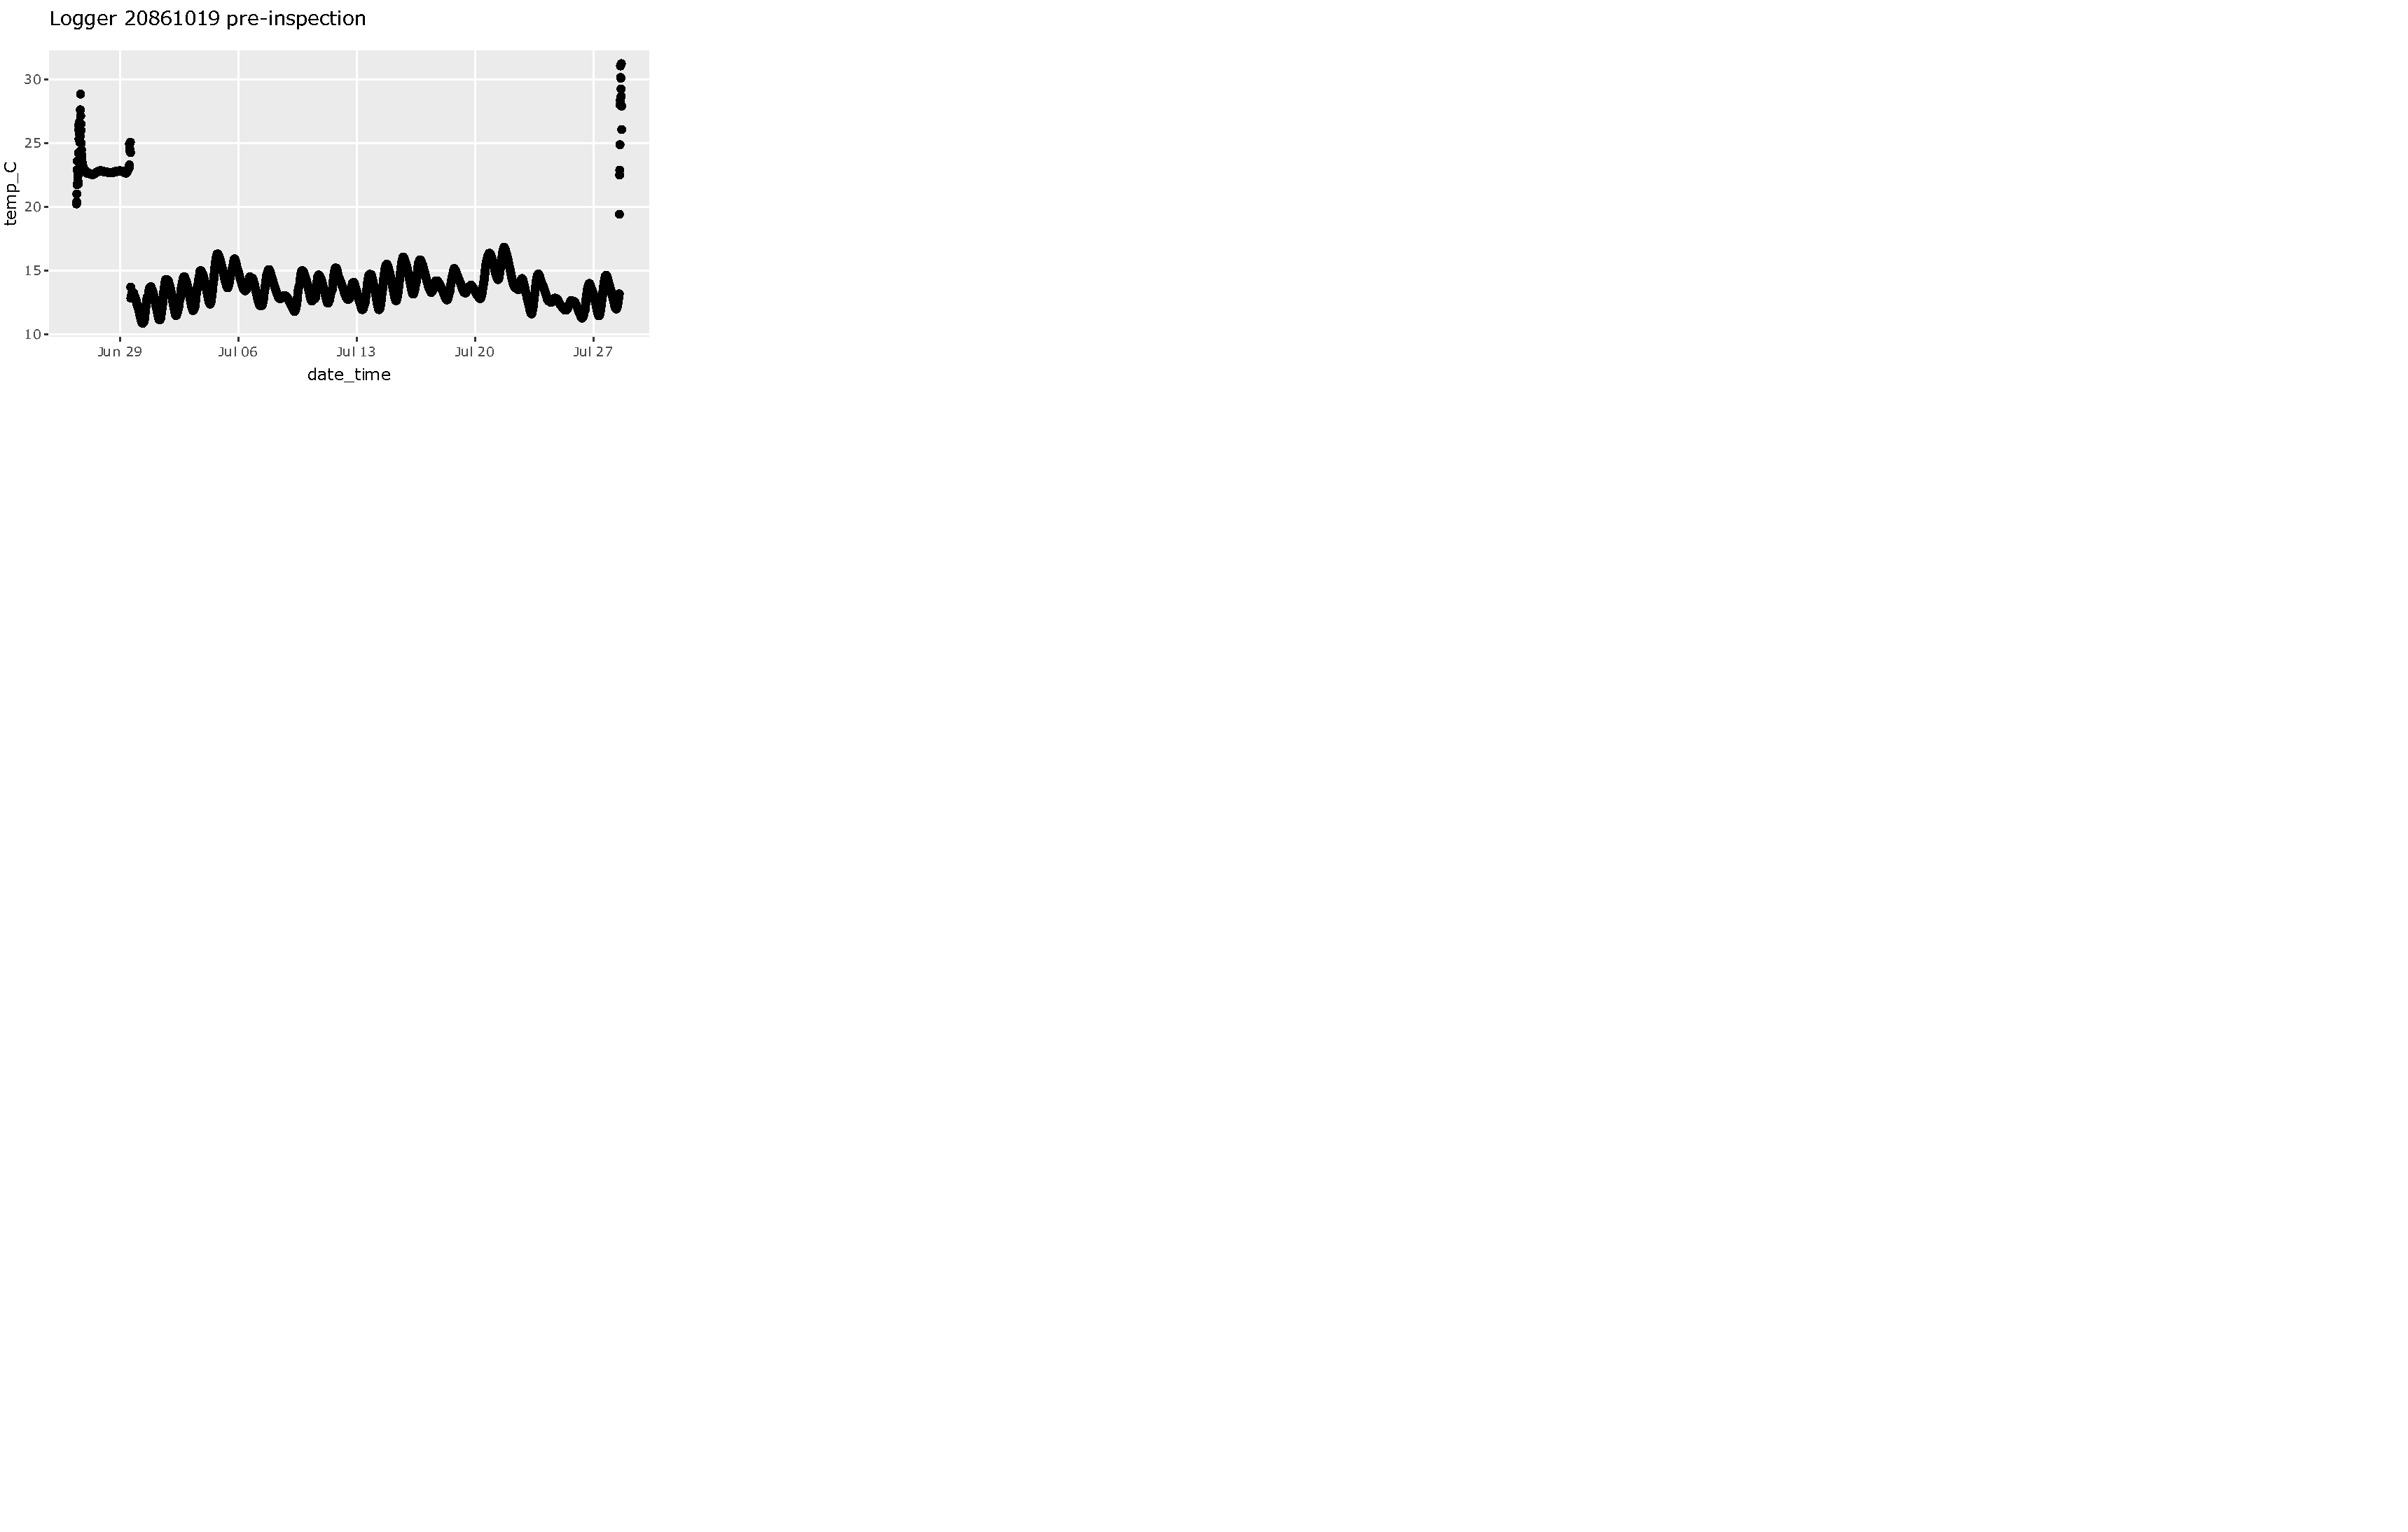
\includegraphics{./temp_logger_data_prep_files/figure-pdf/fig-preqa-1.pdf}

}

\caption{\label{fig-preqa}Example of water temperature time series prior
to quality assurance process}

\end{figure}

\begin{figure}

{\centering 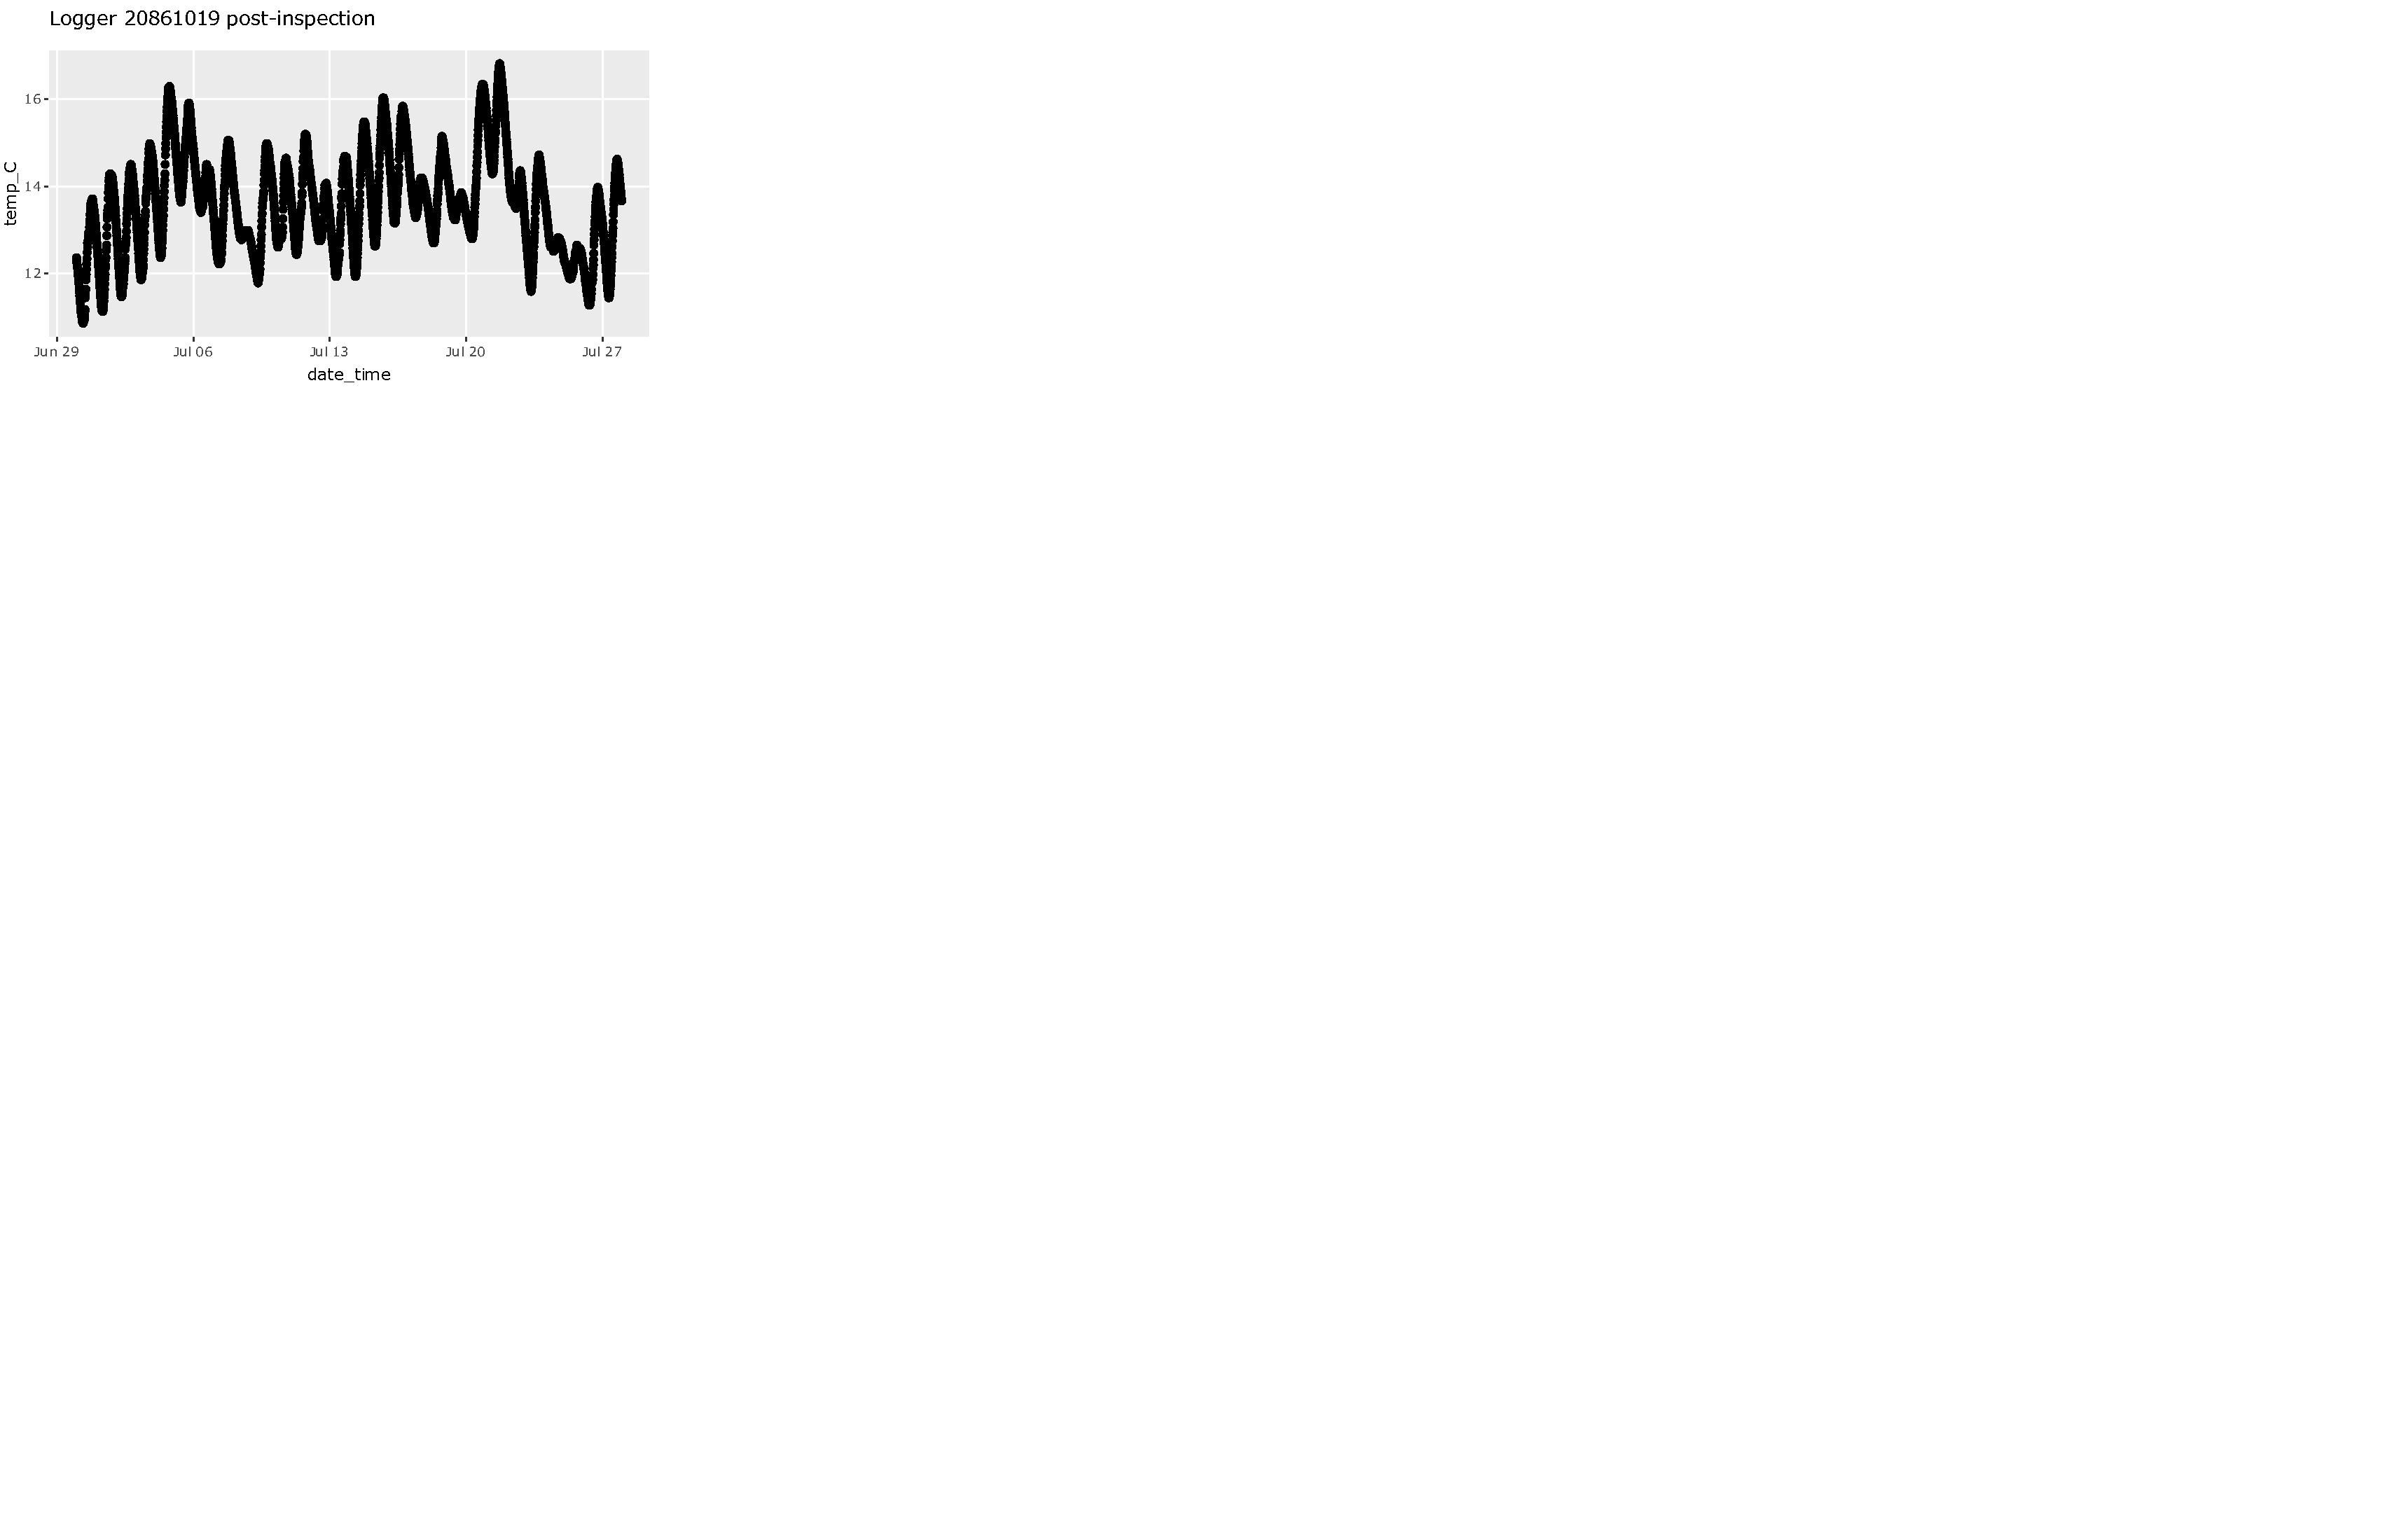
\includegraphics{./temp_logger_data_prep_files/figure-pdf/fig-postqa-1.pdf}

}

\caption{\label{fig-postqa}Example of water temperature time series
after quality assurance inspection}

\end{figure}

\hypertarget{additional-data-preparation-1}{%
\subsection{Additional data
preparation}\label{additional-data-preparation-1}}

The following sections describe additional details on data preparation
specific to each water temperature logger site.

\hypertarget{beaver-creek-1}{%
\subsubsection{Beaver Creek}\label{beaver-creek-1}}

Loggers at the Beaver Creek logger site were deployed in early summer
2020. As part of a separate research project, Alaska Center for
Conservation Science (University of Alaska Anchorage) established a
logger site several hundred meters upstream also in Summer 2020.

We examined if data from the two sites are similar enough to use as a
proxy for each other when data observations are missing. Time series
from both sites are shown in figure Figure~\ref{fig-bc-plots}, and
simultaneous values from both sites are presented in figure
Figure~\ref{fig-bc-reg}.

\begin{figure}

{\centering 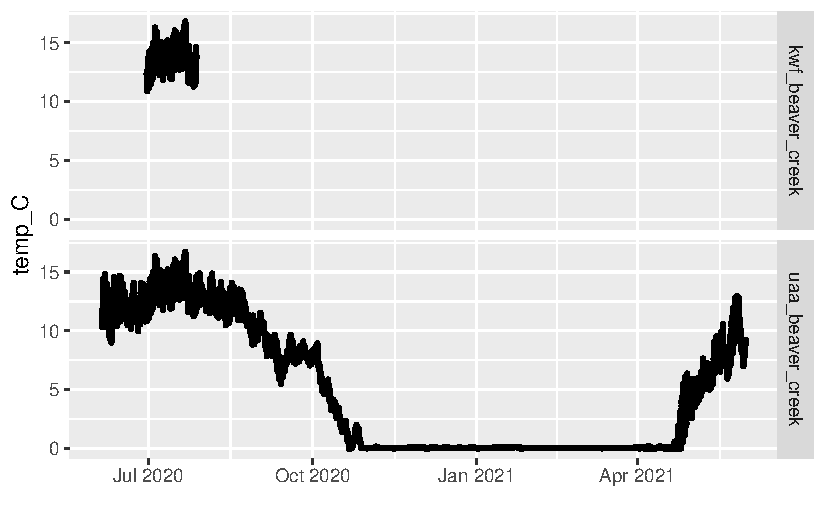
\includegraphics[width=0.7\textwidth,height=0.7\textheight]{./temp_logger_data_prep_files/figure-pdf/fig-bc-plots-1.pdf}

}

\caption{\label{fig-bc-plots}Water temperature time series from Lower
Beaver Creek at two nearby sites.}

\end{figure}

\begin{figure}

{\centering 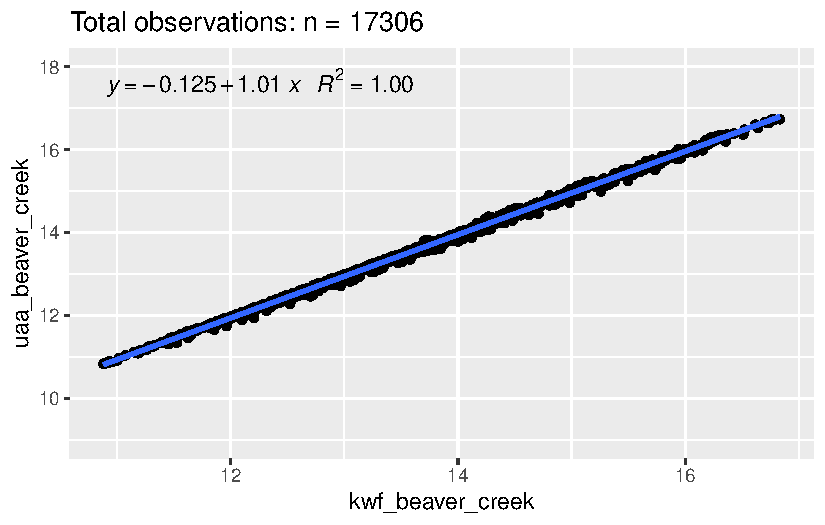
\includegraphics[width=0.7\textwidth,height=0.7\textheight]{./temp_logger_data_prep_files/figure-pdf/fig-bc-reg-1.pdf}

}

\caption{\label{fig-bc-reg}Regression of simultaneous water temperature
observations from two nearby sites in Beaver Creek.}

\end{figure}

The average absolute difference in temperature between the two logger
sites in Beaver Creek is 0.06 ± 0.05 C (mean ± sd). For most
applications, a substitution of data from either of these sites in Lower
Beaver Creek will still accurately represent water temperature.

\hypertarget{lower-crooked-creek}{%
\subsubsection{Lower Crooked Creek}\label{lower-crooked-creek}}

Lower Crooked Creek has two adjacent water temperature monitoring
locations within 20 m of each other. Further details on these two sites
are described below, and figure @fig-cc-map shows locations of the two
sites.

\begin{figure}

{\centering 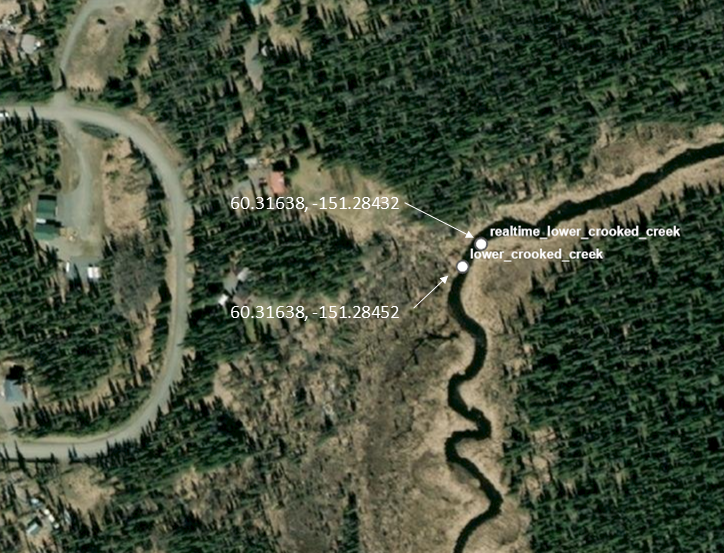
\includegraphics[width=2.41in,height=4.16667in]{./images/lower_crooked_creek_temp_logger_map.png}

}

\caption{\label{fig-cc-map}Lower Crooked Creek temperature monitoring
sites}

\end{figure}

\hypertarget{lower-crooked-creek-real-time-temperature-monitoring-site}{%
\paragraph{Lower Crooked Creek Real-time temperature monitoring
site}\label{lower-crooked-creek-real-time-temperature-monitoring-site}}

Cook Inletkeeper maintains a site installed by Beaded Stream (Anchorage,
AK) that records air and water temperature data in real-time and streams
these data live at
\url{https://inletkeeper.org/our-work/healthy-habitat/real-time-temperature-sites/crooked-creek/}.
Water and air temperature data has been recorded and streamed from this
site at hourly intervals since summer 2017.

Temperature data from this location can be downloaded as a csv file
directly from the above Inletkeeper web link. However, \textbf{\emph{as
of 2022-12-22 there is an error with the publicly available csv file}}.
The publicly available csv file has incorrect time stamps after
12/31/2019. Beaded Stream staff is aware of the error, and says the
remedy will require an in-person visit to the field. In the mean time,
\href{http://www.beadedstream.com/contact/}{contact Beaded Stream staff}
to request access to most current data.

The data with correct time stamps from 2017-08-15 though 2021-10-26,
obtained directly from the internal Beaded Stream dashboard, is also
available for download at this link from GitHub:
\href{https://github.com/Kenai-Watershed-Forum/kenai_thermal_imagery/tree/master/input/real_time_temp_sensor}{\textbf{Download
Lower Crooked Creek Realtime Temperature Data}}.

\hypertarget{lower-crooked-creek-hobo-temppro-v2-logger-site}{%
\paragraph{Lower Crooked Creek HOBO TempPro V2 logger
site}\label{lower-crooked-creek-hobo-temppro-v2-logger-site}}

A pair of HOBO Temp Pro V2 loggers are installed at a location 20 m
upstream from the real-time temperature logger site. Water temperature
is recorded at 15 minute intervals.

During a site visit on 7/28/2021, we discovered that this pair of
loggers potentially resided within a small, previously unidentified cold
water plume incoming from the river-left bank. (On the ArcGIS Online
project map, this feature is identified as ``tributary\_44.'' It was
unclear if the local cold water seep was influencing the loggers in way
such that they would not represent main channel temperature.

In order to determine if HOBO logger data prior to 7/28/2021 is
influenced by the cold seep, we performed the following steps:

\begin{enumerate}
\def\labelenumi{\arabic{enumi}.}
\item
  \emph{Relocated loggers.} On 7/28/2021, we modified logger deployment
  such that one logger was directly upstream of the cold water seep, and
  one remained in its original location within the seep.
\item
  \emph{Compared temperature data upstream vs.~downstream of the seep.}
  We observed consistently cooler temperatures in the downstream logger,
  with an average absolute difference of 1.47 ± 0.30 °C (mean ± sd).
  Figure @fig-cc-plots displays time series from both loggers as well as
  the difference values where simultaneous data from both locations
  exists.
\end{enumerate}

From these data we observe that the small cold water tributary
consistently affected main stem temperature where the loggers recorded
temperature. Temperature contrast was much less apparent in cooler
months, after approximately September 1st, 2021. Thus, the data from
these HOBO loggers prior to 7/28/2021 in the location downstream of the
small cold water tributary should not be considered representative of
main channel Crook Creek temperatures.

We reviewed all paper field forms from the lower Crooked Creek site from
2015 - present
(\href{https://docs.google.com/spreadsheets/d/1jfe6u_xr8-abv8HMxyOm88xEsR4ahYTLGPtztjxSivQ/edit?usp=sharing}{link
here}) to determine the time extent that HOBO loggers may have been
influenced by the cold water tributary. These notes suggest that the
period extended from from 5/31/2019 - 7/28/2021. Prior to 5/31/2019
there is not evidence on file that can confirm whether or not the
loggers were deployed within the cold water plume.

One possible explanation for why technicians failed to observe the cold
water seep when they installed the HOBO loggers in Summer 2019 is that
high discharge level in the Crooked Creek main channel temporarily
masked the localized effect of cold water input. These results highlight
the value of regular site visits to re-verify that the site is
well-mixed, or checking temperatures beyond the minimum of five
observations across a transect.

Additionally, these results exemplify the role of cold water inputs in
maintaining thermal refugia for salmonids in watersheds such as Crooked
Creek. Note in figure Figure~\ref{fig-cc-plots} that water temperature
within the cold water plume in the main channel was often 1.5 °C cooler
than the non-influenced location. Temperature differentials of this
nature help allow salmonids to access a diverse portfolio of thermal
environments important to functions throughout their life cycle such as
migration, metabolism, and foraging.

\begin{figure}

{\centering 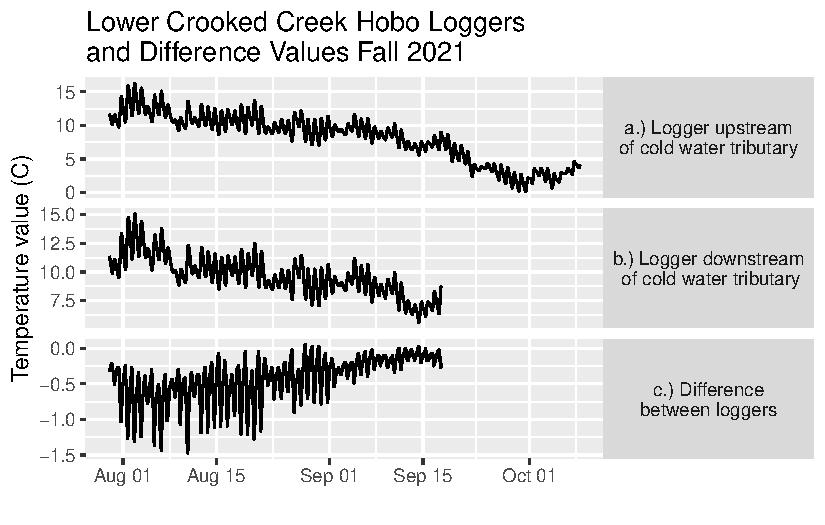
\includegraphics[width=0.7\textwidth,height=0.7\textheight]{./temp_logger_data_prep_files/figure-pdf/fig-cc-plots-1.pdf}

}

\caption{\label{fig-cc-plots}Water temperature time series from Lower
Crooked Creek at two nearby loggers (\textasciitilde3 m apart). a.)
Upstream of a small coldwater tributary, b.) downstream of small
coldwater tributary, c.) difference values between the loggers. Note
different y-axis ranges.}

\end{figure}

\hypertarget{extent-of-water-temperature-time-series}{%
\subsection{Extent of water temperature time
series}\label{extent-of-water-temperature-time-series}}

Figure~\ref{fig-extent-fig} displays temporal extent of currently
available water temperature at each site

\begin{figure}

{\centering 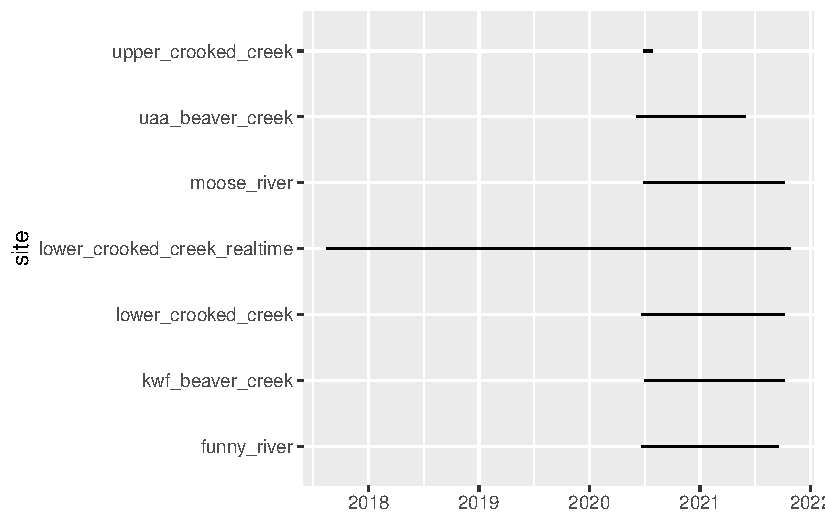
\includegraphics{./temp_logger_data_prep_files/figure-pdf/fig-extent-fig-1.pdf}

}

\caption{\label{fig-extent-fig}Temporal extent of water temperature
logger data}

\end{figure}



\end{document}
